\chapter{Nociones básicas}

Va haber casi infinitas definiciones, así que preparate.

\section{Definición y ejemplos}

\begin{definition}
	Un \emph{espacio métrico} es un par $(X, d)$, donde $X$ es un conjunto y $d: X \times X \to \mathbb{R}_{\geq 0}$ una función llamada \emph{distancia} (o \emph{métrica}), que satisface las siguientes propiedades para todo $x, y, z \in X$:
	\begin{enumerate}
		\item $d(x, y) = 0$ si y sólo si $x = y$.
		\item $d(x, y) = d(y, x)$.
		\item $d(x, z) \leq  d(x, y) + d(y, z)$.
	\end{enumerate}
\end{definition}

\begin{remark}
	Como se cumple la desigualdad triangular, también se cumple
	\begin{itemize}
		\item $d(x_{1}, x_{n}) \leq d(x_{1}, x_{2}) + d(x_{2}, x_{3}) + \dots + d(x_{n-1}, x_{n})$.
		\item $\lvert d(x, z) - d(y, z) \rvert \leq d(x, y)$.
	\end{itemize}
\end{remark}

También tenemos la noción de un subespacio métrico.

\begin{definition}
	Sea $(X, d)$ un espacio métrico y $A \subseteq X$. Se dice que $A$ es un \emph{subespacio métrico} de $X$ si $(A, d_{A \times A})$ es un espacio métrico.
\end{definition}

Veamos algunos ejemplos de espacios métricos.

\begin{example}
	\begin{enumerate}
		\item El espacio $(\mathbb{R}^{n}, \lVert \cdot \rVert_2)$ es un espacio métrico con la norma euclídea, donde la métrica inducida es $d(x, y) = \lVert x - y \rVert_2 = \sqrt{\sum_{i=1}^n (x_i - y_i)^2}$.

		\item Para cualquier conjunto $X$, la métrica discreta está definida por $$d(x, y) = \delta_{xy} = \begin{cases} 0 & \text{si } x = y \\ 1 & \text{si } x \neq y \end{cases}.$$

		\item Si $(X, d)$ es un espacio métrico, entonces
		      \begin{equation*}
			      d'(x, y) = \min(d(x, y), 1)
		      \end{equation*}
		      también es una métrica en $X$, llamada métrica acotada equivalente. Esta métrica garantiza que la distancia entre dos puntos nunca excede $1$.

		\item Si $(V, \langle \cdot, \cdot \rangle)$ es un espacio vectorial con producto interno (sobre $\mathbb{R}$ o $\mathbb{C}$), entonces $\|x\| = \sqrt{\langle x, x \rangle}$ es una norma, y $d(x, y) = \|x - y\|$ es una métrica inducida por la norma. Un ejemplo clásico es el espacio de funciones de cuadrado integrable $L^2([a, b])$ con el producto interno $\langle f, g \rangle = \int_a^b f(x)\overline{g(x)} dx$.

		\item El espacio $C([a, b], \mathbb{R})$ de funciones continuas $f: [a, b] \to \mathbb{R}$. Se pueden definir varias normas en este espacio:
		      \begin{itemize}
			      \item La norma del supremo (o norma $L^\infty$): $\|f\|_\infty = \sup_{x \in [a, b]} |f(x)|$. La métrica inducida es $d(f, g) = \sup_{x \in [a, b]} |f(x) - g(x)|$.
			      \item La norma $L^1$: $\|f\|_1 = \int_a^b |f(x)| dx$. La métrica inducida es $d(f, g) = \int_a^b |f(x) - g(x)| dx$.
			      \item La norma $L^2$: $\|f\|_2 = \left( \int_a^b |f(x)|^2 dx \right)^{1/2}$. La métrica inducida es $d(f, g) = \left( \int_a^b |f(x) - g(x)|^2 dx \right)^{1/2}$.
		      \end{itemize}
		\item El espacio de secuencias $\ell^p$ para $1 \le p < \infty$: $\ell^p = \{ (x_n)_{n=1}^\infty \subset \mathbb{R} : \sum_{n=1}^\infty |x_n|^p < \infty \}$. La norma está definida por $\|x\|_p = \left( \sum_{n=1}^\infty |x_n|^p \right)^{1/p}$. La métrica es $d(x, y) = \|x - y\|_p$.
		\item El espacio de secuencias $\ell^\infty$: $\ell^\infty = \{ (x_n)_{n=1}^\infty \subset \mathbb{R} : \sup_{n \in \mathbb{N}} |x_n| < \infty \}$. La norma es $\|x\|_\infty = \sup_{n \in \mathbb{N}} |x_n|$. La métrica es $d(x, y) = \|x - y\|_\infty$.
	\end{enumerate}
\end{example}

De los ejemplos que di, los más importantes de saber son el espacio de funciones continuas con la norma del supremo y el espacio de secuencias con la norma infinito.


\section{Bolas, abiertos y cerrados}

Vamos a definir los conjuntos básicos que luego vamos a utilizar con mucha frecuencia. Vamos a denotar a un espacio métrico arbitrario con $(X, d)$.

\begin{definition}
	Definimos
	$$
		B(x, r) = \{ y \in X \mid d(x, y) < r\}
	$$
	como la \emph{bola abierta} centrada en $x$ con radio $r$. Análogamente, a
	$$
		\overline{B}(x, r) = \{ y \in X \mid d(x, y) \leq  r\}
	$$
	la \emph{bola cerrada} centrada en $x$ con radio $r$.
\end{definition}

Voy a ir agregando diagramas que ilustren más o menos la idea.

\begin{center}
	\begin{tikzpicture}
	% Dibujar la bola abierta
	\draw[accentcolor, thick, dashed] (0,0) circle (1.5cm);
	\fill[accentcolor!10, opacity=0.7] (0,0) circle (1.5cm);
	\node at (0,0) [fill=black, circle, inner sep=1.5pt, label=below:$x$] {};
	\draw[] (0,0) -- node[above, black] {$r$} (1.5,0);
	\node[above, accentcolor] at (0, 1.8) {Bola Abierta $B(x, r)$};

	% Dibujar la bola cerrada
	\begin{scope}[xshift=4cm]
		\draw[accentcolor, thick] (0,0) circle (1.5cm);
		\fill[accentcolor!10, opacity=0.7] (0,0) circle (1.5cm);
		\node at (0,0) [fill=black, circle, inner sep=1.5pt, label=below:$x$] {};
		\draw (0,0) -- node[above, black] {$r$} (1.5,0); % Línea continua para radio
		\node[above, accentcolor] at (0, 1.8) {Bola Cerrada $\overline{B}(x, r)$};
	\end{scope}
\end{tikzpicture}

\end{center}

¡Ojo! Si bien le decimos ``bola'', el conjunto puede tener una forma totalmente distinta. Por ejemplo, en $\mathbb{R}^2$, pensá qué pasa con las métricas $d_1$, $d_2$ y $d^{\infty}$.

\begin{example}
	Consideremos $C([a, b], \mathbb{R})$ con la norma del supremo. ¿Cómo se ve la bola $B(0, 1)$?

	\begin{center}
		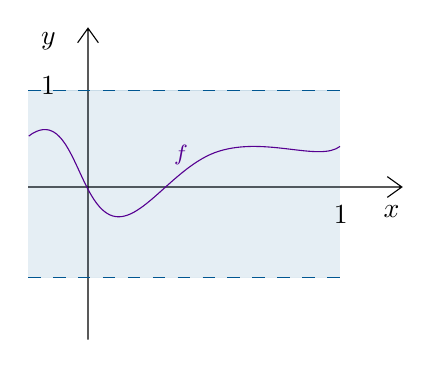
\begin{tikzpicture}[x=0.75pt,y=0.75pt,yscale=-1,xscale=1]
	%uncomment if require: \path (0,300); %set diagram left start at 0, and has height of 300

	%Shape: Axis 2D [id:dp0672040940975357] 
	\draw  (0,76.5) -- (180,76.5)(28.8,0) -- (28.8,150) (173,71.5) -- (180,76.5) -- (173,81.5) (23.8,7) -- (28.8,0) -- (33.8,7)  ;
	%Straight Lines [id:da19847713850781956] 
	\draw [color={rgb, 255:red, 0; green, 86; blue, 145 }  ,draw opacity=1 ][fill={rgb, 255:red, 0; green, 86; blue, 145 }  ,fill opacity=1 ] [dash pattern={on 4.5pt off 4.5pt}]  (0,120) -- (150,120) ;
	%Straight Lines [id:da26723242026257843] 
	\draw [color={rgb, 255:red, 0; green, 86; blue, 145 }  ,draw opacity=1 ][fill={rgb, 255:red, 0; green, 86; blue, 145 }  ,fill opacity=1 ] [dash pattern={on 4.5pt off 4.5pt}]  (0,30) -- (150,30) ;
	%Shape: Rectangle [id:dp7430552976593023] 
	\draw  [draw opacity=0][fill={rgb, 255:red, 0; green, 86; blue, 145 }  ,fill opacity=0.1 ] (0,30) -- (150,30) -- (150,120) -- (0,120) -- cycle ;
	%Curve Lines [id:da49050279449110856] 
	\draw [color={rgb, 255:red, 86; green, 0; blue, 145 }  ,draw opacity=1 ]   (0.23,51.95) .. controls (20.23,36.95) and (23.25,80.01) .. (38,89.21) .. controls (52.75,98.41) and (69.09,66.23) .. (92,59.21) .. controls (114.91,52.18) and (140.23,64.45) .. (150.23,56.95) ;

	% Text Node
	\draw (170,84) node [anchor=north west][inner sep=0.75pt]    {$x$};
	% Text Node
	\draw (5,1) node [anchor=north west][inner sep=0.75pt]    {$y$};
	% Text Node
	\draw (5,22) node [anchor=north west][inner sep=0.75pt]    {$1$};
	% Text Node
	\draw (69,55) node [anchor=north west][inner sep=0.75pt]  [font=\footnotesize,color={rgb, 255:red, 86; green, 0; blue, 145 }  ,opacity=1 ]  {$f$};
	% Text Node
	\draw (146,84) node [anchor=north west][inner sep=0.75pt]    {$1$};


\end{tikzpicture}

	\end{center}

	Como podemos ver, la función $f \in B(0, 1)$ ya que siempre $-1 \leq f(x) \leq 1$, para todo $x \in [0, 1]$. En general, la bola $B(0, 1)$ es el conjunto de funciones que están siempre en esa franja.
\end{example}

A continuación definimos lo que es un entorno de un punto.

\begin{definition}
	Un \emph{entorno} de $x \in X$ es un subconjunto $V \subseteq X$ tal que $x \in V$ y existe una bola $B(x, r) \subseteq V$.
\end{definition}

\begin{center}
	\begin{tikzpicture}
	% The main outer shape (U)
	% Corrected the option syntax: draw/fill options separated from plot options
	\draw[draw=complementarycolor, fill=complementarycolor!10, opacity=0.7] % General draw/fill options
	plot [smooth cycle, tension=0.6]                   % Plot-specific options
	coordinates {
			(1, 1)
			(-2, 1)
			(-1.5, -1)
			(2, -2)
		};
	% Added label for the outer neighborhood set V
	\node[complementarycolor] at (-1.5, 0.5) {$V$};

	% The neighborhood circle (dashed outline and fill)
	\draw[accentcolor, thick, dashed] (0,0) circle (0.5);
	\fill[accentcolor!10, opacity=0.7] (0,0) circle (0.5);

	% The center point x and radius r
	\node at (0,0) [fill=black, circle, inner sep=1.5pt, label=below:$x$] {};
	\draw[] (0,0) -- node[above, black] {$r$} (0.5,0);

	\node[complementarycolor] at (-0.3, 1.75) {Entorno de $x$};
\end{tikzpicture}

























\end{center}

\begin{remark}
	Notemos que $B(x, r)$ siempre es un entorno de $x$.
\end{remark}

\begin{definition}
	Sea $A \subseteq X$. Definimos
	\begin{itemize}
		\item El \emph{interior} de $A$ como
		      $$
			      A^{\circ} = \{ x \in X \mid \exists r > 0 \text{ tal que } B(x, r) \subseteq A\}.
		      $$
		\item La \emph{clausura} de $A$ como
		      $$
			      \overline{A} = \{ x \in X \mid \forall r > 0, B(x, r) \cap A \neq \emptyset\}.
		      $$
		\item La \emph{frontera} de $A$ como
		      $$
			      \partial A = \overline{A} - A^{\circ}.
		      $$
		\item El \emph{exterior} de $A$ como
		      $$
			      \mathrm{ext} A = (X - A)^{\circ}.
		      $$
	\end{itemize}
\end{definition}

\begin{center}
	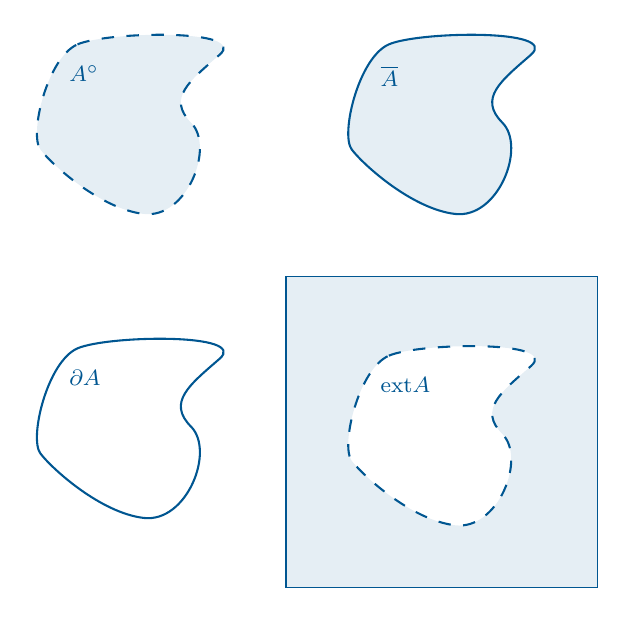
\begin{tikzpicture}[x=0.75pt,y=0.75pt,yscale=-1,xscale=1]
	%uncomment if require: \path (0,300); %set diagram left start at 0, and has height of 300

	%Shape: Polygon Curved [id:ds678130924119981] 
	\draw  [color={rgb, 255:red, 0; green, 86; blue, 145 }  ,draw opacity=1 ][fill={rgb, 255:red, 0; green, 86; blue, 145 }  ,fill opacity=0.1 ][dash pattern={on 4.5pt off 4.5pt}][line width=0.75]  (49.56,38.17) .. controls (64.04,31.89) and (132.48,30.63) .. (118,43.2) .. controls (103.53,55.77) and (92.59,64.15) .. (104.25,75.88) .. controls (115.91,87.61) and (102.23,122.38) .. (81.41,119.87) .. controls (60.58,117.36) and (37.36,96.23) .. (31.71,88.87) .. controls (26.05,81.5) and (35.08,44.45) .. (49.56,38.17) -- cycle ;
	%Shape: Polygon Curved [id:ds19735692429512375] 
	\draw  [color={rgb, 255:red, 0; green, 86; blue, 145 }  ,draw opacity=1 ][fill={rgb, 255:red, 0; green, 86; blue, 145 }  ,fill opacity=0.1 ][line width=0.75]  (199.56,38.17) .. controls (214.04,31.89) and (282.48,30.63) .. (268,43.2) .. controls (253.53,55.77) and (242.59,64.15) .. (254.25,75.88) .. controls (265.91,87.61) and (252.23,122.38) .. (231.41,119.87) .. controls (210.58,117.36) and (187.36,96.23) .. (181.71,88.87) .. controls (176.05,81.5) and (185.08,44.45) .. (199.56,38.17) -- cycle ;
	%Shape: Polygon Curved [id:ds4025351553833618] 
	\draw  [color={rgb, 255:red, 0; green, 86; blue, 145 }  ,draw opacity=1 ][line width=0.75]  (49.56,184.63) .. controls (64.04,178.34) and (132.48,177.09) .. (118,189.66) .. controls (103.53,202.23) and (92.59,210.6) .. (104.25,222.34) .. controls (115.91,234.07) and (102.23,268.84) .. (81.41,266.33) .. controls (60.58,263.82) and (37.36,242.69) .. (31.71,235.32) .. controls (26.05,227.96) and (35.08,190.91) .. (49.56,184.63) -- cycle ;
	%Shape: Path Data [id:dp28607428735171037] 
	\draw  [draw opacity=0][fill={rgb, 255:red, 0; green, 86; blue, 145 }  ,fill opacity=0.1 ][dash pattern={on 4.5pt off 4.5pt}] (300,150) -- (300,300) -- (150,300) -- (150,150) -- (300,150) -- cycle (199.56,188.17) .. controls (185.08,194.45) and (176.05,231.5) .. (181.71,238.87) .. controls (187.36,246.23) and (210.58,267.36) .. (231.41,269.87) .. controls (252.23,272.38) and (265.91,237.61) .. (254.25,225.88) .. controls (242.59,214.15) and (253.53,205.77) .. (268,193.2) .. controls (282.48,180.63) and (214.04,181.89) .. (199.56,188.17) -- cycle ;
	%Shape: Square [id:dp6423377198062709] 
	\draw  [color={rgb, 255:red, 0; green, 86; blue, 145 }  ,draw opacity=1 ] (150,150) -- (300,150) -- (300,300) -- (150,300) -- cycle ;
	%Shape: Polygon Curved [id:ds7262645597364767] 
	\draw  [color={rgb, 255:red, 0; green, 86; blue, 145 }  ,draw opacity=1 ][dash pattern={on 4.5pt off 4.5pt}][line width=0.75]  (199.56,188.17) .. controls (214.04,181.89) and (282.48,180.63) .. (268,193.2) .. controls (253.53,205.77) and (242.59,214.15) .. (254.25,225.88) .. controls (265.91,237.61) and (252.23,272.38) .. (231.41,269.87) .. controls (210.58,267.36) and (187.36,246.23) .. (181.71,238.87) .. controls (176.05,231.5) and (185.08,194.45) .. (199.56,188.17) -- cycle ;

	% Text Node
	\draw (44.33,47.33) node [anchor=north west][inner sep=0.75pt]  [font=\footnotesize,color={rgb, 255:red, 0; green, 86; blue, 145 }  ,opacity=1 ]  {$A^{\circ }$};
	% Text Node
	\draw (194.33,47.33) node [anchor=north west][inner sep=0.75pt]  [font=\footnotesize,color={rgb, 255:red, 0; green, 86; blue, 145 }  ,opacity=1 ]  {$\overline{A}$};
	% Text Node
	\draw (44.33,193.79) node [anchor=north west][inner sep=0.75pt]  [font=\footnotesize,color={rgb, 255:red, 0; green, 86; blue, 145 }  ,opacity=1 ]  {$\partial A$};
	% Text Node
	\draw (194.33,197.33) node [anchor=north west][inner sep=0.75pt]  [font=\footnotesize,color={rgb, 255:red, 0; green, 86; blue, 145 }  ,opacity=1 ]  {$\mathrm{ext} A$};


\end{tikzpicture}

\end{center}

Establecidos los conceptos de interior y clausura, podemos definir los conjuntos abiertos y cerrados.

\begin{definition}
	Sea $A \subseteq X$. Decimos que
	\begin{itemize}
		\item $A$ es \emph{abierto} si $A^{\circ} = A$.
		\item $A$ es \emph{cerrado} si $\overline{A} = A$.
	\end{itemize}
\end{definition}

\begin{remark}
	Hay que tener cuidado con $\overline{B}(x, r)$ y $\overline{B(x, r)}$, ya que no necesariamente son iguales. Lo que sí vale es que $\overline{B(x, r)} \subseteq \overline{B}(x, r)$
\end{remark}

\begin{proposition}
	Sea $A \subseteq X$. Entonces,
	\begin{itemize}
		\item $A^\circ \subseteq A \subseteq \overline{A}$.
		\item $(A^\circ)^\circ = A^\circ$, $\overline{\overline{A}} = \overline{A}$.
		\item $\overline{A \cup B} = \overline{A} \cup \overline{B}$, $(A \cap B)^\circ = A^\circ \cap B^\circ$.
	\end{itemize}
\end{proposition}

\begin{proof}
	No voy a demostrarlo, pero pensá por qué tiene sentido esto. (Mira los diagramas de arriba.)
\end{proof}

La siguiente proposición es extremadamente útil.

\begin{proposition}
	Sea $\{ A_i \}_{i \in I}$ una familia de abiertos. Entonces,
	\begin{enumerate}
		\item La unión $\bigcup_{i \in I} A_i$ es abierta.
		\item Si $I$ es finito, entonces la unión $\bigcap_{i \in I} A_i$ es abierta.
	\end{enumerate}
\end{proposition}

\begin{proof}
	\framebox{1.} Sea $U = \bigcup_{i \in I} A_i$. Si $x \in U$, entonces existe un $i \in I$ tal que $x \in A_i$. Por lo tanto, existe una bola $B(x, r)$ que cumple que $B(x, r) \subseteq A_i \subseteq U$. Por lo tanto, $U \subseteq U^{\circ}$. Entonces, $U$ es abierto.

	\framebox{2.} Sea $I$ finito y $V = \bigcap_{i \in I} A_i$. Si $x \in V$, entonces $x \in A_i$ para todo $i \in I$. Por lo tanto, existen bolas $B(x, r_i) \subseteq A_i$ para todo $i \in I$. Definimos $r = \min_{i \in I} r_i$, entonces $B(x, r) \subseteq \bigcap_{i \in I} A_i = V$. Por lo tanto, $V \subseteq V^{\circ}$. Entonces, $V$ es abierto.
\end{proof}

La proposición análoga para cerrados vale intercambiando las intersecciones por uniones y \textit{viceversa}.

\begin{proposition}
	Sea $\{ A_i \}_{i \in I}$ una familia de cerrados. Entonces,
	\begin{enumerate}
		\item La intersección $\bigcap_{i \in I} A_i$ es cerrado.
		\item Si $I$ es finito, entonces la intersección $\bigcup_{i \in I} A_i$ es cerrado.
	\end{enumerate}
\end{proposition}

\begin{proof}
	\framebox{1.} Sea $C = \bigcap_{i \in I} A_i$. Queremos demostrar que $C$ es cerrado. Equivalentemente, demostraremos que su complemento $C^c$ es abierto. Tenemos que $C^c = (\bigcap_{i \in I} A_i)^c = \bigcup_{i \in I} A_i^c$. Como cada $A_i$ es cerrado, su complemento $A_i^c$ es abierto. Por la Proposición anterior (parte 1), la unión de una familia arbitraria de abiertos es abierta. Por lo tanto, $C^c = \bigcup_{i \in I} A_i^c$ es abierto. En consecuencia, $C = \bigcap_{i \in I} A_i$ es cerrado.

	\framebox{2.} Sea $I$ finito y $D = \bigcup_{i \in I} A_i$. Queremos demostrar que $D$ es cerrado. Equivalentemente, demostraremos que su complemento $D^c$ es abierto. Tenemos que $D^c = (\bigcup_{i \in I} A_i)^c = \bigcap_{i \in I} A_i^c$. Como cada $A_i$ es cerrado, su complemento $A_i^c$ es abierto. Por la Proposición anterior (parte 2), la intersección de una familia finita de abiertos es abierta. Por lo tanto, $D^c = \bigcap_{i \in I} A_i^c$ es abierto. En consecuencia, $D = \bigcup_{i \in I} A_i$ es cerrado.
\end{proof}


\section{Densos}

\begin{definition}
	Sea $A \subseteq X$. Decimos que $A$ es \emph{denso} (en $X$) si $\overline{A} = X$.
\end{definition}

\begin{remark}
	Otra formulación equivalente es que para todo $U \subseteq X$ abierto no vacío se cumple que $A \cap U \neq \varnothing$.
\end{remark}

El ejemplo típico de subconjunto denso es $\mathbb{Q}$ en $\mathbb{R}$. (Agarramos el punto medio entre dos puntos de $\mathbb{R}$ y lo truncamos en algún momento para que esté en $\mathbb{Q}$.)

\begin{definition}
	Sea $A \subseteq X$. Se dice que $x \in X$ es un \emph{punto de acumulación} de $A$ si
	\begin{center}
		para todo $\varepsilon > 0$, $\left| B(x, \varepsilon) \cap A \right| \geq \aleph_0$.
	\end{center}
	El conjunto
	$$
		A' = \{ x \in X \mid x \text{ es un \emph{punto de acumulaci\'on} de } A \}
	$$
	se llama el \emph{conjunto derivado} de $A$.
\end{definition}

\begin{center}
	\begin{tikzpicture}
	% Define the start and end points for the line
	\coordinate (start) at (0,0);
	\coordinate (end) at (6,0); % Adjust 6 for desired length of the line

	% Mark 0
	\node[below] at (start) {$0$};
	\draw (start) -- +(0,2.5mm); % Tick mark for 0



	\node[below] at (1/2,0) {$\dots$};
	\draw (1/2,0) -- +(0,2.5mm); % Tick mark for 1/3


	\node[below] at (6/6,0) {$\frac{1}{6}$};
	\draw (6/6,0) -- +(0,2.5mm); % Tick mark for 1/3

	% % Mark 1/3
	% Calculate position: 1/3 of the total length (6 units) is 2 units
	\node[below] at (6/5,0) {$\frac{1}{5}$};
	\draw (6/5,0) -- +(0,2.5mm); % Tick mark for 1/3

	% Mark 1/3
	% Calculate position: 1/3 of the total length (6 units) is 2 units
	\node[below] at (6/4,0) {$\frac{1}{4}$};
	\draw (6/4,0) -- +(0,2.5mm); % Tick mark for 1/3


	% Mark 1/3
	% Calculate position: 1/3 of the total length (6 units) is 2 units
	\node[below] at (6/3,0) {$\frac{1}{3}$};
	\draw (6/3,0) -- +(0,2.5mm); % Tick mark for 1/3

	% Mark 1/2
	% Calculate position: 1/2 of the total length (6 units) is 3 units
	\node[below] at (6/2,0) {$\frac{1}{2}$};
	\draw (6/2,0) -- +(0,2.5mm); % Tick mark for 1/2

	% Mark 1
	\node[below] at (end) {$1$};
	\draw (end) -- +(0,2.5mm); % Tick mark for 1
\end{tikzpicture}

\end{center}

\begin{remark}
	Notemos que $\overline{A} = A \cup A'$.
\end{remark}


\section{Distancia a conjuntos}

\begin{definition}
	Sea $x \in X$ y $A \subseteq X$. Definimos la \emph{distancia} entre $x$ y $A$ como
	$$
		d(x, A) = \inf_{a \in A} d(x, a).
	$$
\end{definition}

\begin{remark}
	Se cumple la desigualdad triangular con conjuntos. O sea,
	$$
		d(x, A) \leq d(x, y) + d(y, A).
	$$
\end{remark}

\begin{definition}
	Sean $A, B \subseteq X$ no vacíos. Definimos la \emph{distancia} entre $A$ y $B$ como
	$$
		d(A, B) = \inf_{a \in A, b \in B} d(a, b).
	$$
\end{definition}

Y una última definición.

\begin{definition}
	Sea $A \subseteq X$. Definimos el \emph{diámetro} de $A$ como
	$$
		\diam(A) = \sup_{a, b \in A} d(a, b).
	$$
\end{definition}

A menudo nos va a servir la siguiente proposición.

\begin{proposition}
	Sea $A \subseteq X$ y $x \in X$. Entonces,
	\begin{equation*}
		d(x, A) = 0 \quad \text{ si y sólo si } \quad x \in \overline{A}.
	\end{equation*}
\end{proposition}

\begin{proof}
	($\Rightarrow$) Supongamos que $d(x, A) = 0$. Consideramos una bola $B(x, r)$ con $r > 0$. Como $d(x, A) = 0$, existe un $a \in A$ tal que $d(x, a) < r$. Por lo tanto, $B(x, r) \cap A \neq \varnothing$. Por lo tanto, $x \in \overline{A}$.

	($\Leftarrow$) Supongamos que $x \in \overline{A}$. Entonces, para toda bola $B(x, \frac{1}{n})$ con $n \in \mathbb{N}$, existe $a_n \in A$ tal que $d(x, a_n) < \frac{1}{n}$. Por lo tanto, consideramos a $d(a_n, x) \longrightarrow 0$. Entonces, $d(x, A) = 0$.
\end{proof}


